\chapter{调制识别的深度框架研究}

\section{引言}

尽管机器学习的目的是提供一种通用的问题解决算法,但目前性能最优的网络模型大部分仍然是对应于特定应用的。
目前存在几种较完善的网络,比如包括多层感知机、RNN、CNN及其许多变体等,
他们被应用在各个领域,取得了很好效果\cite{lecun2015deep, schmidhuber2015deep}。
然而,由于模型所面对的环境不同,数据不同,数据分布也不同;
因此,其他领域的很多模型对于调制识别任务并不一定完全适应,需要进行相应的探索。 \par

在第三章中,基于深度网络框架的层面,提出了一种不同类型深度模型融合的深度网络框架,
并将其应用到无线信号调制识别任务中,而且取得了一定的性能提升。
在本章中,将以LeCun的经典五层网络结构\cite{lecun1998gradient}为基准,
从网络底层研究网络超参数对调制识别性能的影响,
并从模型的方差与偏差\cite{周志华2016机器学习}、欠拟合与过拟合\cite{goodfellow2016deep}等角度来理解出现这些现象的原因。\par

\section{系统模型}

在大部分现有的深度神经网络中,卷积层是它们共有的基本网络单元。
每个卷积层由若干个卷积核组成,每个卷积核通常非常小($1 \times 1$到$5 \times 5$是图像处理中的常见尺寸)。
在传统的DSP应用中,卷积核通常设计得非常宽,而非设计成很深的多层结构。
计算机视觉领域中,神经网络的一个明显趋势是建立更深的网络来学习更复杂的函数变换和层次特征关系。\par

标准的卷积层传递函数在方程\eqref{eqt_5_1}中给出:
\begin{equation}
	\label{eqt_5_1}
	f(I_i) = f (b_j + \sum_{i}(k_{ij} * I_i))
\end{equation}
其中,$f(I_i)$是第$i$个卷积核的输出特征图(Featrue Map),
$b$和$k$表示卷积核的偏置和卷积核的权重参数,$I_i$代表卷积核的输入 值,$*$ 表示卷积运算,
并且$f(\dots)$表示诸如ReLU单元或Sigmoid单元等激活函数。\par

本章中,假设所有的网络结构都是基于图\ref{fig_5_0}的框架,基准的CNN在Softmax分类层之前有两个卷积层和一个全连接层,Softmax层之后输出样本分类结果。\par
\begin{figure}[!htbp]
	\centering
	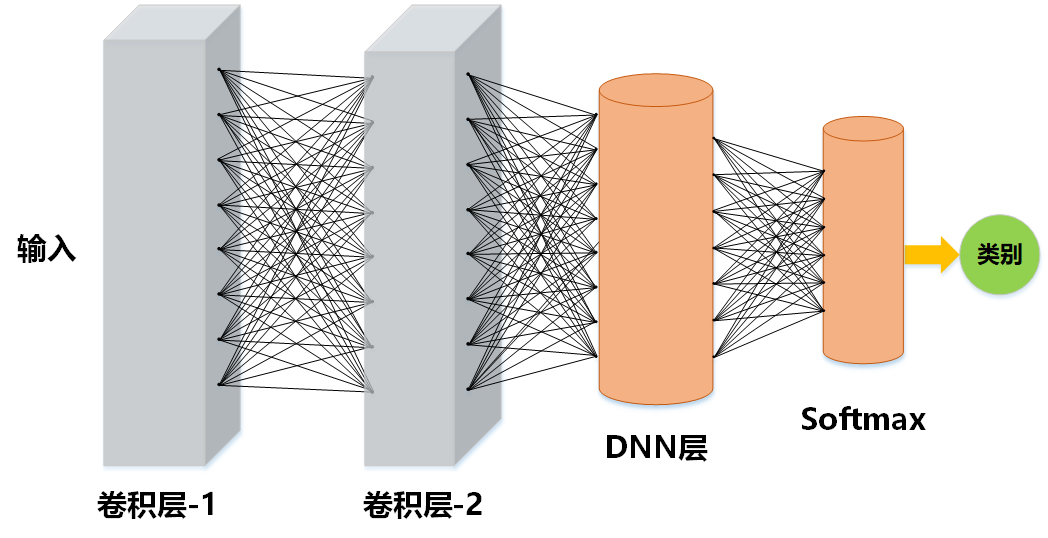
\includegraphics[scale=0.6]{figures/chapter_5/fig_5_0}
	\caption{本章所用CNN网络框架}
	\label{fig_5_0}
\end{figure}

整个网络中,所变化的只是网络的层数、卷积核的高度和宽度、卷积核的数目等这几个超参数。
所有的模型训练都将使用Adam优化器,因为它提供了梯度归一化和动量的方法,
降低了像学习率这样的超参数对模型训练结果的影响。
每个卷积层和隐藏层都使用整流线性单元(ReLU)作为激活函数,并使用dropout=0.5来降低模型的过拟合,
而预测时,使所有的单元处于激活状态。\par

\subsection{模型的偏差与方差}
\label{sec_5_2_1}
偏差恒量机器学习算法对于输入样本的期望输出与真实值的偏离程度,本质上表征了机器学习算法本身的拟合能力。
方差表示算法性能随训练集的变化而产生的波动,本质上表征了数据扰动所对算法性能的影响。
噪声则表示当前任务下训练数据与数据的真实值之间的差距,即任何学习算法所能达到的期望泛化误
差的F下界,衡量了学习任务本身的难度。\par

假设调制识别的训练样本集为$X$,$Y$为训练样本的真实类别。
对于训练集中的每一个样本$x_i \in X$,假设其真实类别为$\hat{y_i}$,$y_i$为在训练集中的类别。
在训练集$X$上学得模型$\phi(\dots)$,$\phi(x_i; X)$为输入样本为$x_i$时的输出,即预测类别:
\begin{equation}
	\label{eqt_5_2}
	y_i = \phi(x_i), x_i \in X
\end{equation}

假设网络预测的期望为:
\begin{equation}
	\label{eqt_5_3}
	\overline{\phi}(x) = E_X\left[ \phi(x; X) \right]
\end{equation}
如果使用相同数目的不同训练样本集$\hat{X}$进行训练,那么有训练集的方差:
\begin{equation}
	\label{eqt_5_4}
	\delta_{\hat{X}}^2(x) = E_{\hat{X}}\left[ (\phi(x, \hat{X}) - \overline{\phi}(x))^2\right]
\end{equation}

此时,模型的噪声为$\epsilon^2 = E_{\hat{X}}\left[ (\hat{y} - y)^2\right]$,
表示训练数据与真实数据的误差情况。
模型的期望输出与真实标记的差别为偏差,即:
\begin{equation}
	bias^2(x) = (\overline{\phi}(x)  - \hat{y})^2
\end{equation}
假设噪声期望为$0$,即$E_{\hat{X}}[\hat{y} - y] = 0$,则可知泛化误差为偏差、方差与噪声之和:
\begin{equation}
	E(\phi; X) = bias^2(x) + \delta_{\hat{X}}^2(x) + \epsilon^2
\end{equation}

为了简化模型的分析,假设所有的训练样本都是无偏的,
即对于任意训练样本$(x_i, y_i) \in X$,有$\hat{y}_i \equiv y_i$。此时可得泛化误差$E(\phi; X) $:
\begin{equation}
	E(\phi; X) = bias^2(x) + \delta_{\hat{X}}^2(x) 
\end{equation}

因此,可以从降低偏差和方差的角度出发,来提升模型的性能。

\subsection{过拟合与欠拟合}

在训练机器学习模型时,通常以降低训练误差为目标,获得模型的参数。
通常,我们不仅希望学习算法在训练集上表现良好,更希望其在非训练的数据集上同样具备良好的性能。
泛化正是衡量机器学习算法在未知数据上表现能力良好的一种定性标准。
泛化误差可以定义为模型对于新输入未知样本的误差期望。
欠拟合是指模型不能在训练集上获得足够低的误差,而过拟合是指测试误差大于训练误差。\par

模型的容量是指模型的拟合能力。
容量较低的模型其拟合能力较弱 ,很难反映训练集的数据分布。
容量高的模型,由于其拟合能力过强,可能会将噪声数据也学习到模型中,从而发生过拟合。
为了控制模型的过拟合或者欠拟合程度,可以通过调整模型的容量来实现。\par

通过小节\ref{sec_5_2_1}中的结果可知,
模型的泛化性能是由学习算法本身的拟合能力、数据的充分性以及学习任务本身的难度共同决定的。

对于给定的学习任务$T$,为了取得较好的泛化性能,需要使模型具备较低的偏差,即模型可以充分拟合训练数据,
并且还要使模型的方差处于较小值,即使得数据扰动对模型产生的影响尽量小。\par

然而,实际中偏差与方差却具备相反的倾向性。
对算法进行训练时,
如果训练不足, 则机器学习模型的拟合能力不够强,训练数据的扰动不足以使模型产生显著变化
,此时偏差主导了泛化误差;
而随着训练程度的加深,模型的拟合能力逐渐增强,训练数据产生的扰动逐渐能被模型所学习,
此时方差逐渐主导了泛化误差;
在训练程度达到临界条件以后,如验证误差超过了训练误差一定阈值,模型的拟合能力已经非常强,
训练数据发生的轻微扰动都会导致模型发生显著的变化,
此时,模型可能学习到训练数据某些样本自身的、非全局性的特性,这就会产生模型的过拟合。\par

\section{网络超参数对调制识别的影响}
网络的超参数,如学习速率,每层卷积核的数量,卷积核的大小以及卷积层的数目等,
会影响网络规模,特征提取的数目等,如果不具备一定的领域先验知识很难优化。\par

本节将研究网络卷积核以及卷积层等相关超参数对分类性能的影响,
这可以为后续的研究提供一定的网络整体架构的参考,节省了后续研究的时间成本,
并有助于进一步探究新的网络底层架构,以提升调制识别的性能。\par

\subsection{网络层数对调制识别的影响}
在调制识别场景中应用的是宽度较小的卷积核,由于小卷积核无法获取全局特征,
此问题可以通过增加网络层数来解决。
多层卷积核的局部感知野逐渐叠加后,较深层的卷积核的局部感知野也会逐渐扩大,
进而学得全局特征。因此,卷积层的深度,在一定程度上决定了网络的拟合能力。\par

(1)卷积层数目变化超参数\par

本小节将对网络层数对调制识别的影响进行探索。
由于本节中仅对卷积层深度对分类性能的影响进行探索,而且网络的训练本身是一个非常耗时的过程,
所以,为了降低时间成本并简化分析提供一个定性的结果,本小节中的仿真所有卷积核数目都为$32$,
并将卷积核的大小从$1\times3$到$1\times12$变化。\par
网络层次深度对训练数据遍历次数的要求差别很大,
为了解决这个问题,本小节中将所有的网络epoch设置为一个较大值(本文中epoch=500),
以满足那些对于复杂网络对于较高次数epoch训练的需求。
同时,本节中将使用预停止策略:
假设训练过程中,训练损失在$N_{pre\_stop}$(本小节中设置为$N_{pre\_stop}=10$)个epoch内不降低,
即在这段训练时间范围内,模型不能得到很好的优化,此时则停止训练。
这样可以在尽量保证准确率的同时提高训练效率。\par

(2)卷积层数变化对分类性能的影响\par

根据本节定义的超参数,对调制识别系统进行仿真,结果如图\ref{fig_5_1}所示。\par
\begin{figure}[!h]
	\centering
	\subfloat[3D展示]{
		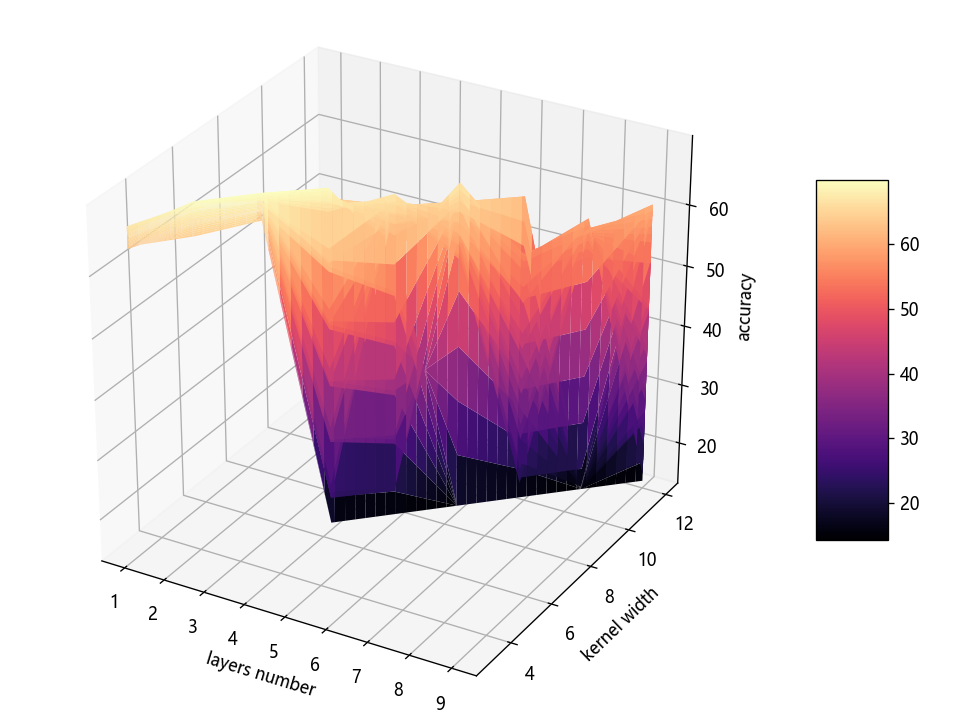
\includegraphics[width=0.52\linewidth, height=0.41\linewidth]{figures/chapter_5/fig_5_1}
		\label{fig_5_1_a}}
	\subfloat[热力图展示]{
		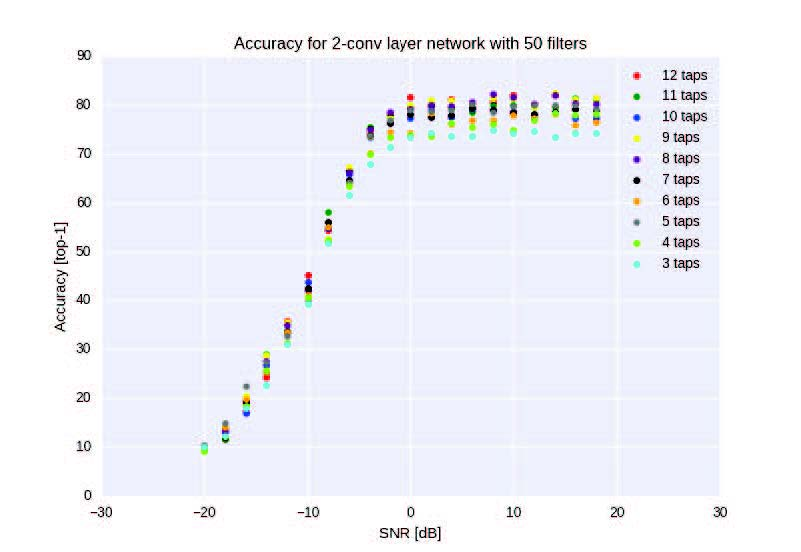
\includegraphics[width=0.48\linewidth, height=0.4\linewidth]{figures/chapter_5/fig_5_2}
		\label{fig_5_1_b}}
	\caption{不同卷积核宽度下,卷积层数目对分类准确率的影响}
	\label{fig_5_1}
\end{figure}

通过图\ref{fig_5_1}可以发现,分类性能具有一个相对整体性的趋势:
当卷积层大于3时,分类准确率几乎成下降趋势。
通过图\ref{fig_5_1_a}可以观察到,系统性能在卷积层为$3$,卷积核的宽度为$6$以上时,
系统性能能够达到一个较高的水准;
同时可以看到卷积核宽度较大时,
卷积核层数在大于$3$时分类准确率几乎呈一个断崖式下跌。\par

在图\ref{fig_5_1_b}中可以清楚地发现,整幅图像在卷积层数目较大、卷积核数目较小时,系统的性能较差。
卷积层数目小于4时,系统性能随卷积核宽度变化不大,增大卷积核宽度并不能很大程度上提升系统分类性能;
卷积层较大时,增加卷积层的宽度反而会降低系统性能。\par

接下来,以卷积层数目作为变量,观察不同卷积核宽度条件下的分类性能,结果如图\ref{fig_5_2}。
\begin{figure}[!h]
	\centering
	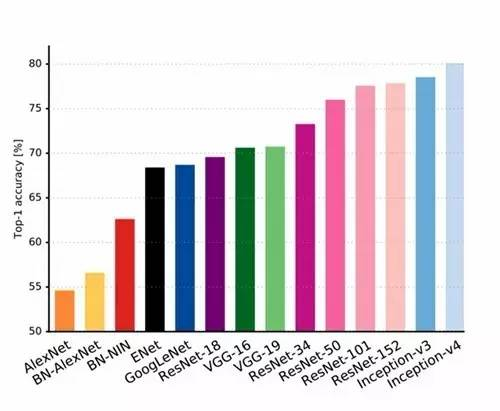
\includegraphics[scale=0.6]{figures/chapter_5/fig_5_4}
	\caption{分类准确率随卷积层数目和卷积核宽度的变化}
	\label{fig_5_2}
\end{figure}

从图\ref{fig_5_3}可以发现,整体而言,不同卷积核宽度的平均分类准确率,随着卷积层数目增加,
首先先轻微地上升,然后出现较大幅度的下降。\par

增加卷积层的深度,在卷积层数目$N_{layers} \leq 3$时,可以微小地改善分类性能。
当卷积层深度$N_{layers} \geq 4$时,改变卷积层的数量在分类准确率几乎都呈下降趋势;
但是,不同卷积核宽度的网络性能下降程度不同,
卷积核宽度较大的网络越,随着卷积层深度的增大性能下降程度较低。
在卷积层深度$N_{layers} \leq 3$时,可以发现分类性能几乎随着卷积核宽度的增加而增加,
直到卷积核宽度达到$11$时,达到分类性能的上限;
同时,分类性能在此时随着卷积层数增加而增加。\par

(3)卷积层对系统性能影响的分析\par

在卷积层数较低时,分类性能有所增加,
这可能是因为模型的拟合能力不足以完全表征信号的特性。
在卷积层数$N_{layers} \geq 4$时,网络性能大幅下降;
因为卷积核宽度较大时,分类性能仍然处于一个较高的水准,而且分类性能会随着卷积层数目的增加而发生剧烈的突变,
所以可以确定此时导致分类性能下降的主要原因是网络的训练难度增加;
其次,网络性能在卷积层数目为3时达到了性能的最高点,之后性能一直呈下降趋势,
这是网络发生过拟合的一个节点。
这表明对于本文所用的数据集而言,可能是由于调制数据通常只改变正弦曲线的幅度,频率或相位,
因此对于调制方式而言数据的复杂度并不高,没有必要学习更高层次的深度特征。
\par

\subsection{卷积核数目对调制识别的影响}
CNN是通过增加网络的深度来增强拟合能力的,而网络对于数据特征的提取,
主要是通过不同的卷积核进行参数学习得到的,卷积核的数目在一定程度上表征了网络所能学习特征的数目,
即网络对数据理解的维度高低。\par
上一小节对卷积层数目对调制识别的影响进行了探讨,本节将对网络结构进行更细化的研究,
探索卷积核数目对调制识别的影响。\par
(1)卷积核变化超参数\par
由第三章可知,第一层卷积核为$1 \times 7$,第二层卷积核为$2 \times 6$时,分类器具备较好的性能。
因此,在本小节中,所有的仿真都基于这样的卷积核结构进行,变化的仅仅是卷积核的数目。
由于训练神经网络时间成本较高,很难对每一个卷积核数目参数进行遍历,
所以本节中选择一些有代表性的参数进行试验,主要目的是定性的分析卷积核数目的变化对于分类性能的影响。
定义卷积核数目集合$\kappa =\{16, 32, 48, 64,  96, 128, 196, 256\}$,
第一个卷积层与第二个卷积层的卷积核数目,分别从集合$\kappa$中按照卷积核数目由小到大选取,
卷积核变化范围为16 \textasciitilde 256。
这样两个卷积层的核数目组合共有$|\kappa|^2=64$种,
即网络训练时总的遍历次数为$|\kappa|^2$次,复杂度为$O(n^2)$。
同时使用自适应学习速率的Adam优化器进行训练,同样设置较大的epoch并应用预停止策略,来探索卷积核数目对分类性能的影响。\par

(2)卷积核数目变化对分类性能的影响\par

通过对不同卷积核数目组合的网络进行训练,最终得到分类器性能随卷积核数目变化的情况。
图\ref{fig_5_3}显示了两个卷积层中卷积核数量从16增加到256时,样本分类准确率的变化情况。\par
\begin{figure}[!h]
	\centering
	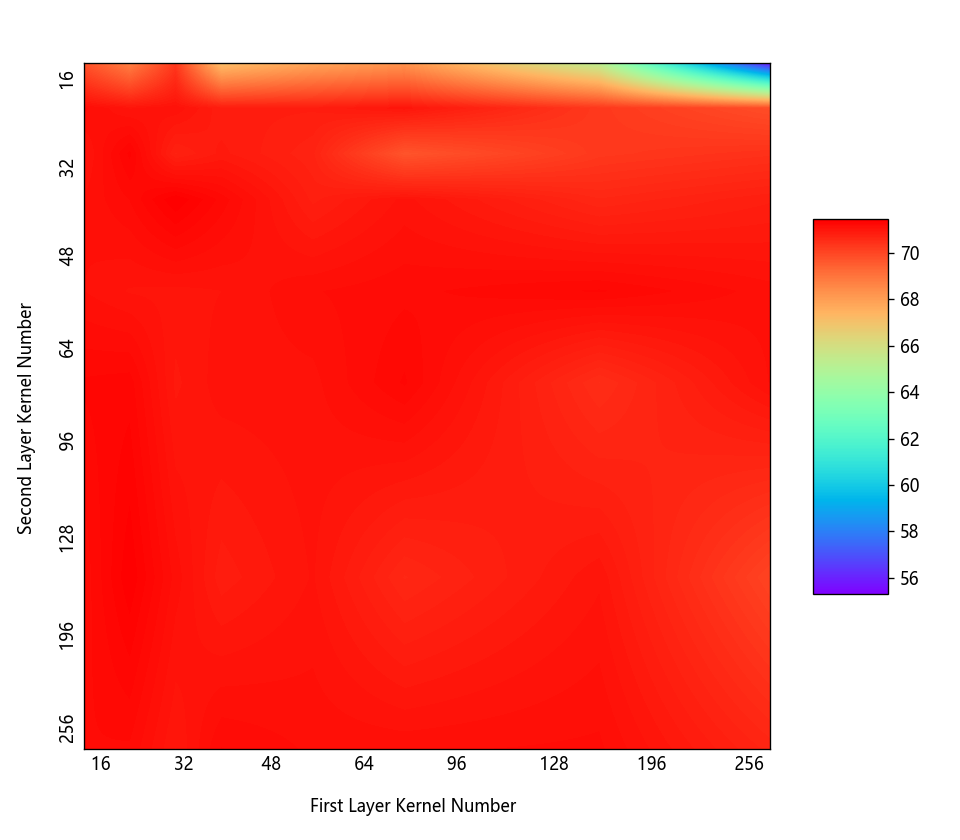
\includegraphics[width=0.7\linewidth, height=0.6\linewidth]{figures/chapter_5/fig_5_10}
	\caption{分类准确率随卷积核数目的变化情况}
	\label{fig_5_3}
\end{figure}

通过图\ref{fig_5_3}可以发现,在第一层卷积核数目为$16$,即第一层卷积核数目较小时,
网络的性能几乎随着第二层卷积核数目的增大而减小。
而随着第一层卷积核增大,改变第二层卷积核数目,系统分类准确率变化很小,只有轻微的波动。
由于本小节所用的是较小的卷积核,因此单卷积层的卷积核的局部感知野有限,
因此通过增加卷积层的数目来增大卷积核的局部感知野。
当第一个卷积层的卷积核数目较小时,网络所学得的特征图的数目也相对较少,
而此时增大第二个卷积层的卷积核数目,由于第二层卷积核本身所能感知的信息较多,
由于第一个卷积层提取的信息量有限,因此第二层很难得到有效训练。
所以,当第一个卷积层中卷积核数目较小时网络性能的下降主要是因为网络本身训练难度增加所致。\par

图\ref{fig_5_4}中,以第一个卷积层中卷积核数目为横轴,展示第一层和第二层卷积核数目变化对分类性能的影响。\par
\begin{figure}[!h]
	\centering
	\subfloat{
		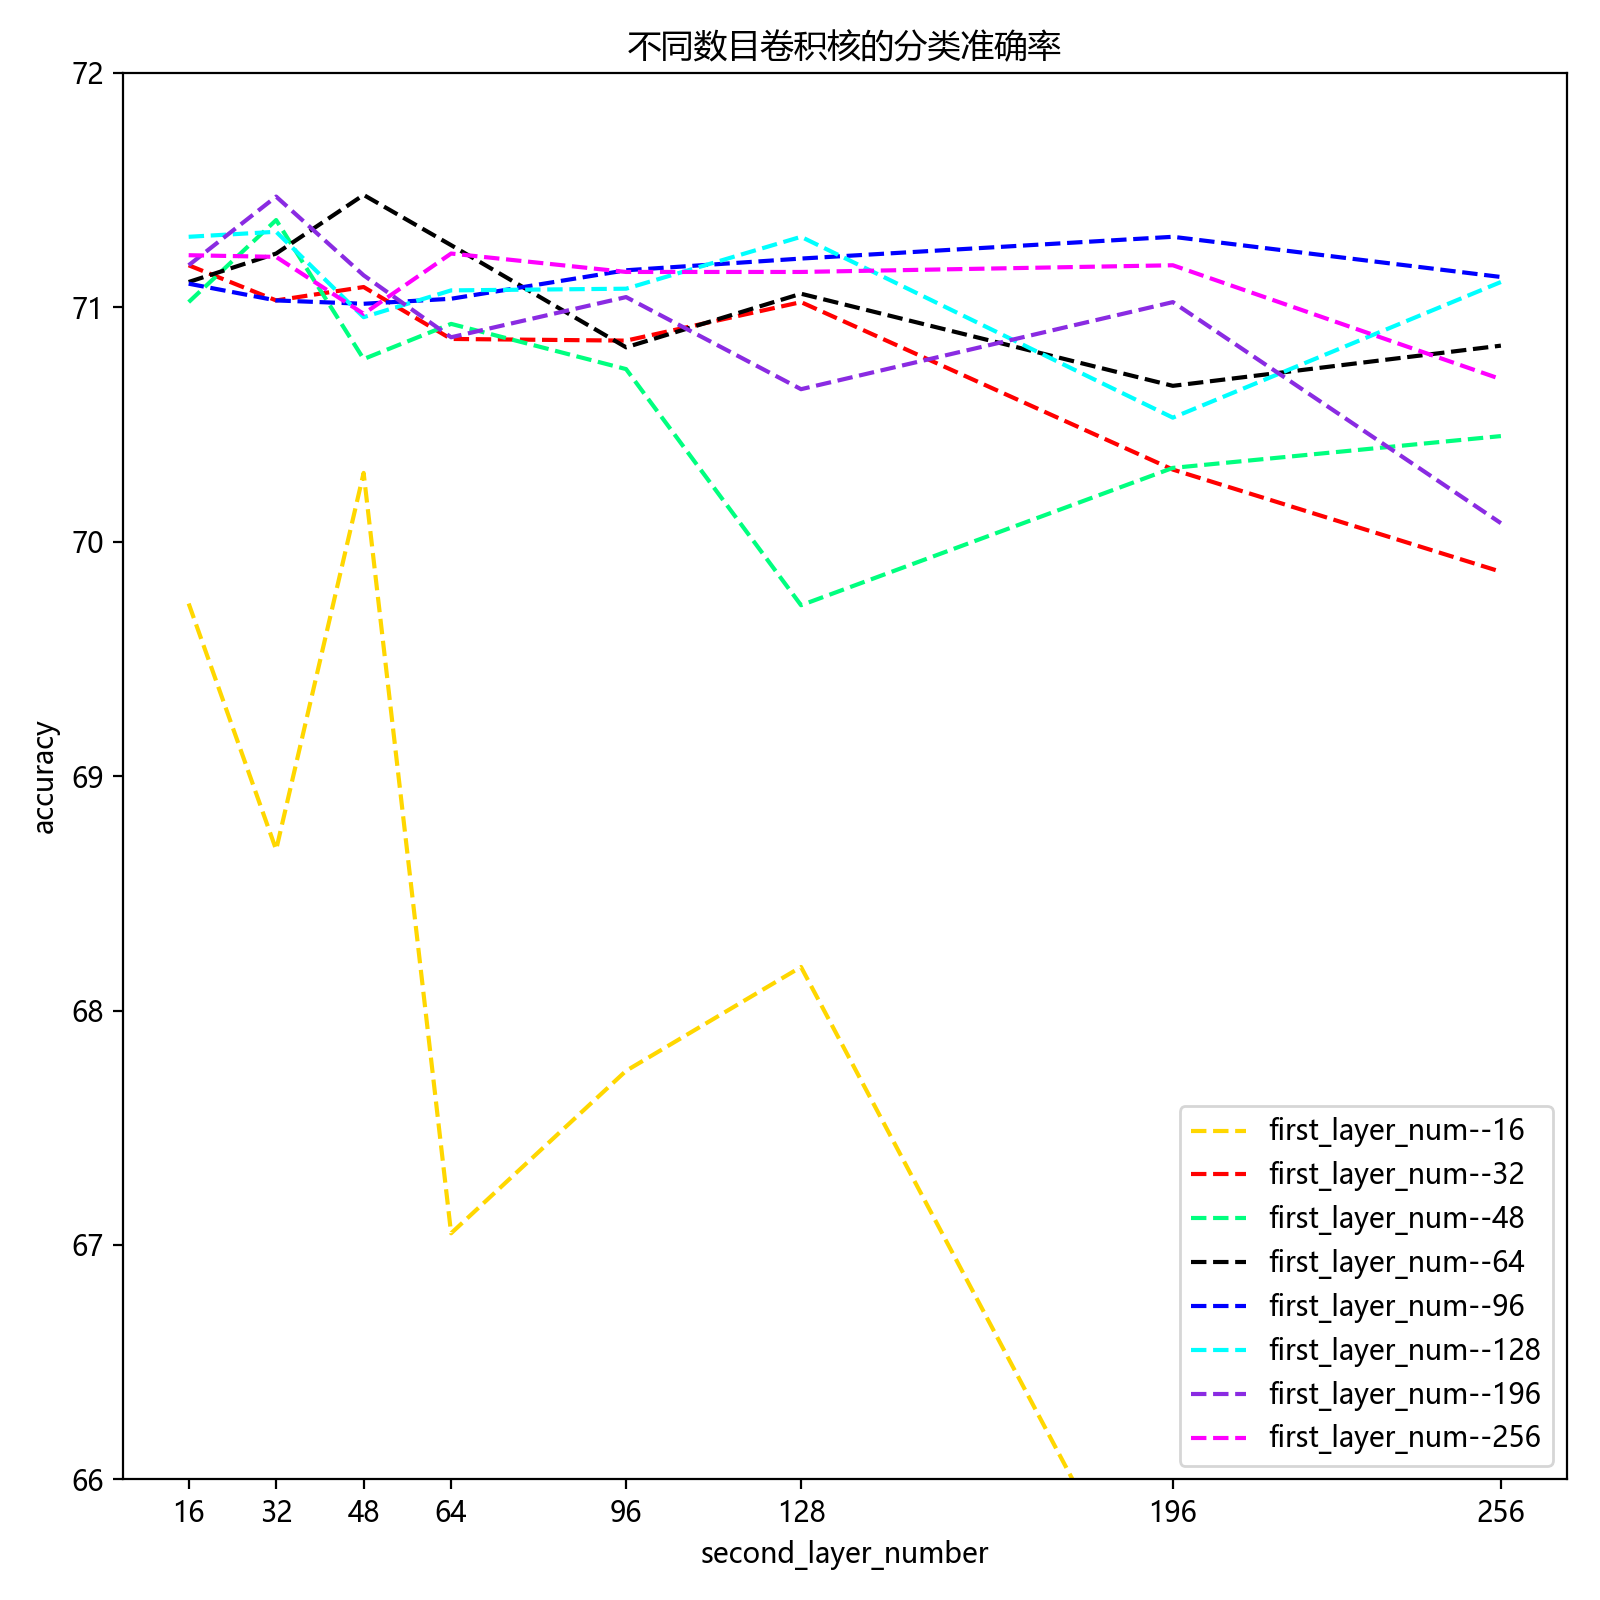
\includegraphics[width=0.5\linewidth, height=0.42\linewidth]{figures/chapter_5/fig_5_11}
		\label{fig_5_4_a}}
	\subfloat{
		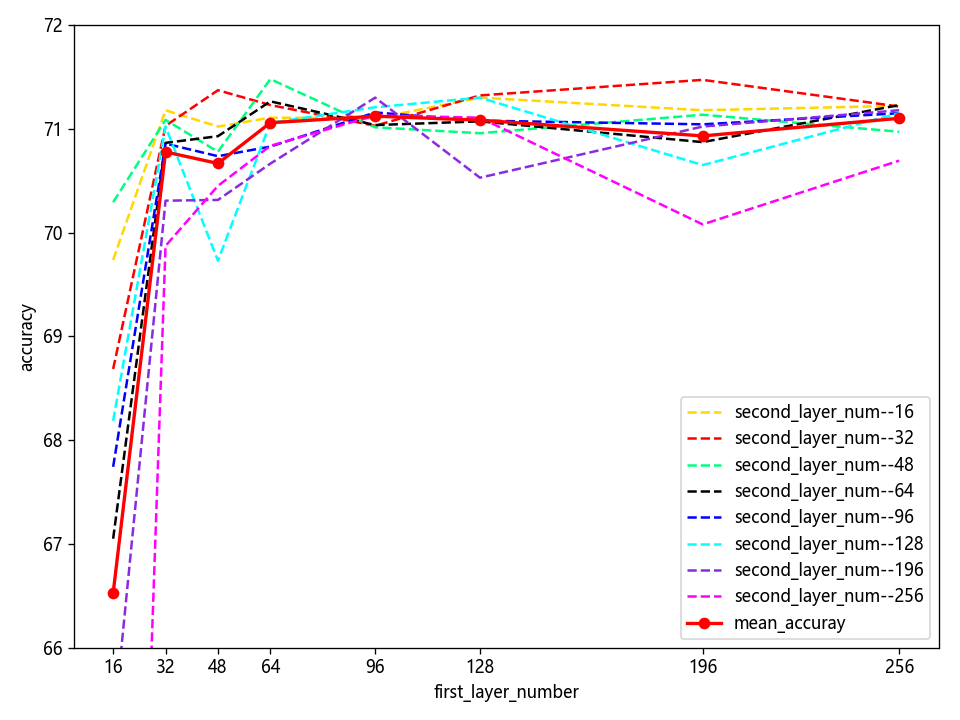
\includegraphics[width=0.5\linewidth, height=0.42\linewidth]{figures/chapter_5/fig_5_12}
		\label{fig_5_4_b}}
	\caption{第一卷积层中卷积核数目对分类准确率的影响}
	\label{fig_5_4}
\end{figure}
从图\ref{fig_5_4_a}可知第一卷积层中卷积核数目$N_{kernel}^{(1)} \leq 32$时,
系统性能会随着第二层中卷积核的数目变化而发生较大的波动;
而当$N_{kernel}^{(1)} \geq 48$时,第二个卷积层中卷积核数目变化对系统性能影响较小。
这可能是由于在第一层卷积核数目较小时,偏差主导了模型的泛化性能。\par

从图\ref{fig_5_4_b}可以发现,第一卷积层中卷积核数目$N_{kernel}^{(1)} \leq 32$时,
第二层卷积核数目的变化与性能没有明确的相关关系,
但是,整体而言,第二层的卷积核数目在$N_{kernel}^{(2)} \leq 48$时能取得较好的性能。
而在第一个卷积层数目$N_{kernel}^{(1)} \geq 48$时,系统性能波动较大,
此时可能是模型训练时的鞍点等因素所致。
当以第一层卷积核数目作为自变量,第二层所有数目卷积核分类准确率的均值作为因变量时,
即图\ref{fig_5_4_b}中红色的粗线,可以发现其整体上准确率呈先上升后下降的趋势,
系统性能在$N_{kernel}^{(1)} = 64, N_{kernel}^{(2)} =64$时取得最优。
\par

\begin{figure}[!h]
	\centering
	\subfloat{
		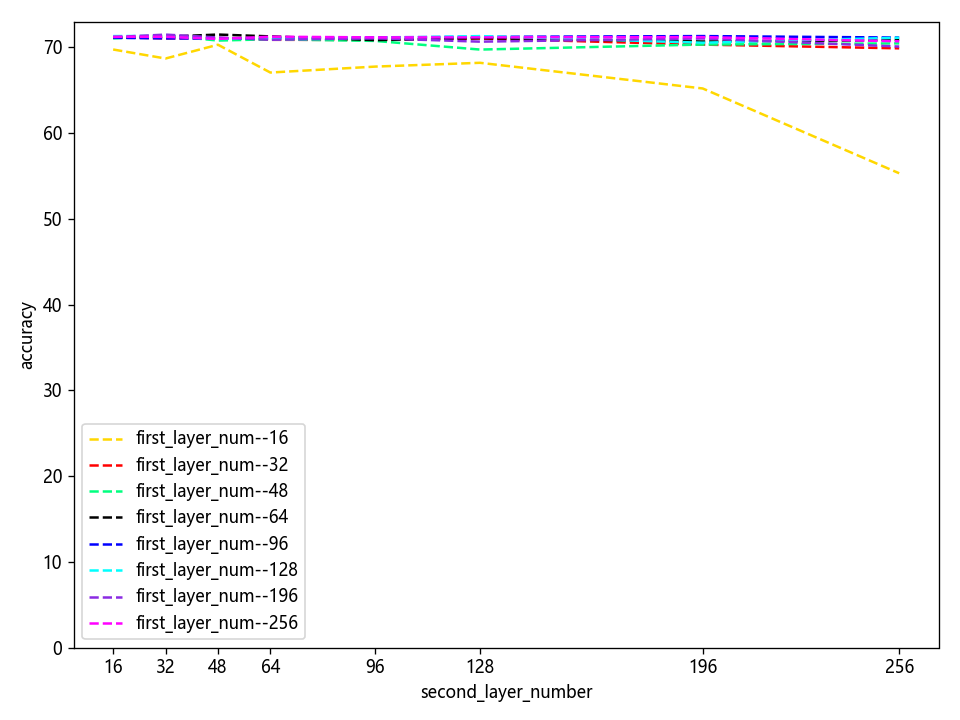
\includegraphics[width=0.5\linewidth, height=0.42\linewidth]{figures/chapter_5/fig_5_13}
		\label{fig_5_5_a}}
	\subfloat{
		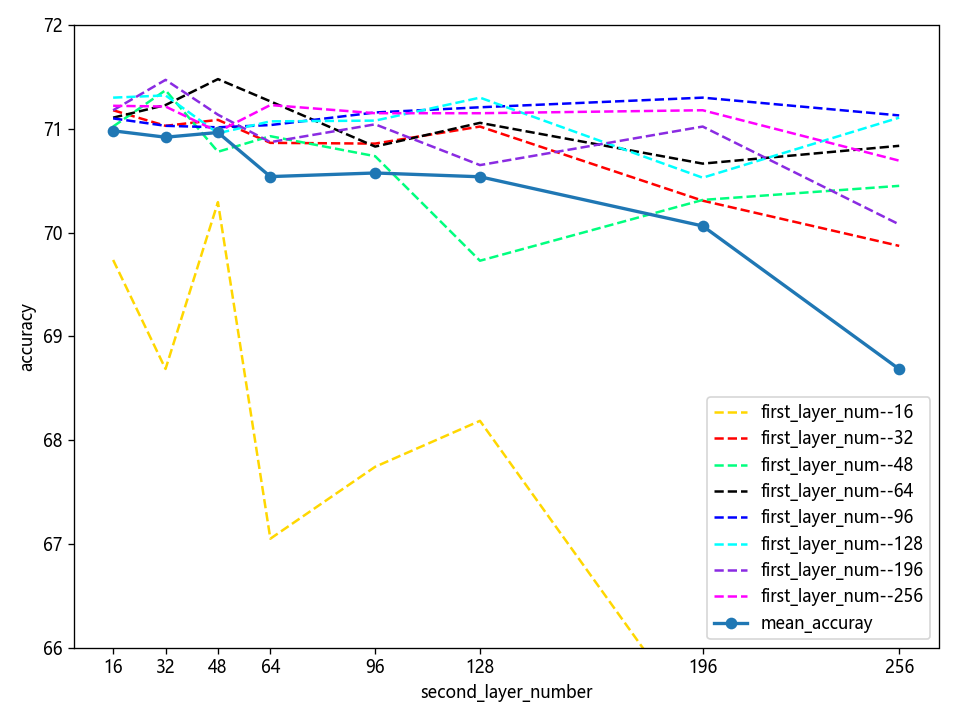
\includegraphics[width=0.5\linewidth, height=0.42\linewidth]{figures/chapter_5/fig_5_14}
		\label{fig_5_5_b}}
	\caption{第二卷积层中卷积核数目对分类准确率的影响}
	\label{fig_5_5}
\end{figure}
从图\ref{fig_5_5_a}中可以发现,分类性能整体随着第二卷积层数目的增加而下降。
而且,当第一卷积层中卷积核数目为$16$时,性能下降的最为明显。
图\ref{fig_5_5_b}中可以更清楚的看到,当第一层卷积核数目较小时,
系统性能随着第二卷积层中卷积核数目的增加而下降得很明显,而且波动幅度较大;
从平均准确率而言,可以发现图中粗的红色实线也是呈下降趋势,
即系统整体性能几乎是随着第二卷积层数目的增加而下降的。
\par
(3)卷积核对系统性能影响的分析\par
由于网络本身的深度较小,当卷积核数目很小时,受限于卷积核数目的限制,特征提取的数目也相应的较少,很难较完整地反映数据本身的特征,分类准确率的上限会出于一个较低值。当卷积核数目增加,相当于特征数目也在相应的增加,这样,网络本身的拟合能力增强,卷积核所提取的卷积特征能更好地反映数据的内在特征,因此,分类性能的上界相应提高,可以获得较好的分类结果。\par
当卷积核的数目增大到一定的程度,网络的拟合能力过强,不仅能够拟合出数据本身的性质,同时将一些异常点也进行了拟合,这就造成了过拟合;同时,由于数据量有限,也很难将网络参数训练到一个较优的水平。因此,网络的分类性能可能会随着卷积核数目的增加而降低。\par

由于不同卷积层中的卷积核局部感知野不同,越深度的卷积核相对而言观察的信息范围更广,因此,更深层次的卷积层中卷积核数目应该相对较少;如果较深层的卷积核数目大于较浅层中卷积核数目,模型就容易发生过拟合现象。

\subsection{卷积核大小对调制识别的影响}
在CNN中,特征提取的过程从底层卷积核到高层卷积核,层层接收局部的输入,最后不断聚合。
对于卷积核而言,卷积核的高度$height$和宽度$width$决定了卷积核感知野的范围。
对于卷积层的高度而言,训练样本是一个$2\times128$的时间序列,
可以看成是由两个$128$维的向量组成。
其中,第一行表示信号的实部,第二行为信号的虚部。
这样,在利用卷积核对信号进行卷积特征提取时,如果卷积核的宽度为$1$,
相当于是在信号的实部或者虚部进行采样值的卷积运算;
如果卷积核的宽度为$2$表示我本不仅对信号进行实部的运算,同时考虑到了信号的虚部,
这样进行卷积时,可能同时会包含信号的能量信息。
本小节将探究不同卷积核的高度和宽度对调制识别性能的影响。\par

(1)卷积核宽度对分类性能影响的3D展示\par

借鉴第三章采用的CNN结构,将第一个卷积层的卷积核数目固定在$64$,
将第二个卷积层的卷积核数目固定在$32$,因为这种情况下网络具有较好的分类性能。
假设卷积核高度$H^{(1)}$和$H^{(2)}$在$1$与$2$之间变化,
卷积核的宽度$W^{(1)}$和$W^{(2)}$在$3$到$9$之间变化。
则总的训练迭代次数为$8 \times 8 \times 2 \times 2 = 256$。
同样,网络训练时使用Adam优化器,并采用预停止策略,最后分类结果如图\ref{fig_5_6}所示。\par
\begin{figure}[!h]
	\centering
	\subfloat[$H^{(1)} = 1, H^{(2)} = 1$]{
		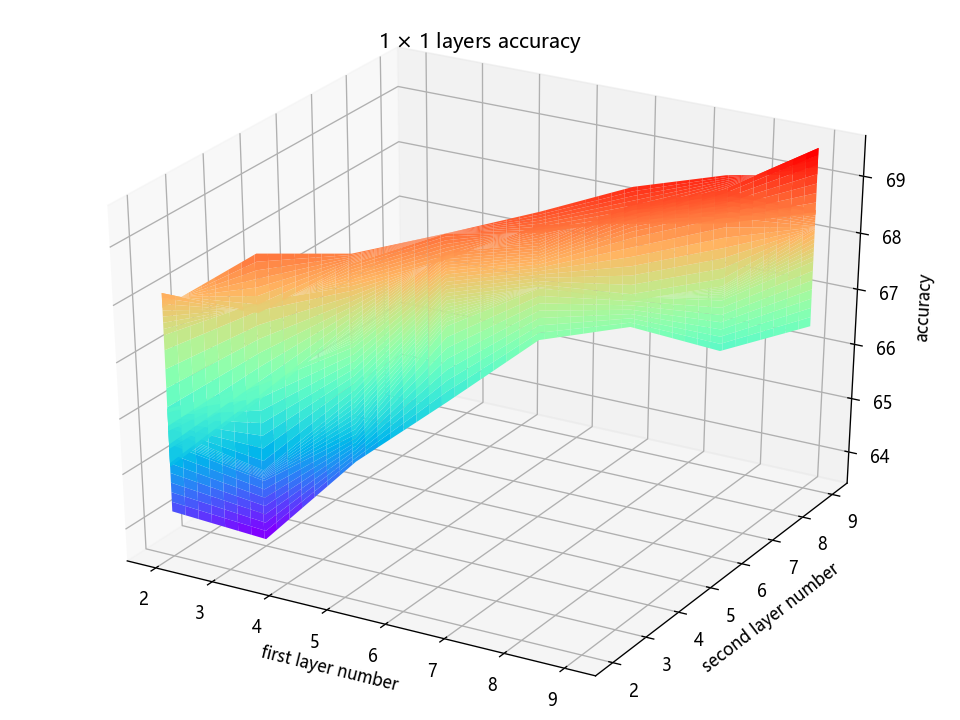
\includegraphics[width=0.5\linewidth, height=0.4\linewidth]{figures/chapter_5/fig_5_15}
		\label{fig_5_6_a}}
	\subfloat[$H^{(1)} = 1, H^{(2)} = 2$]{
		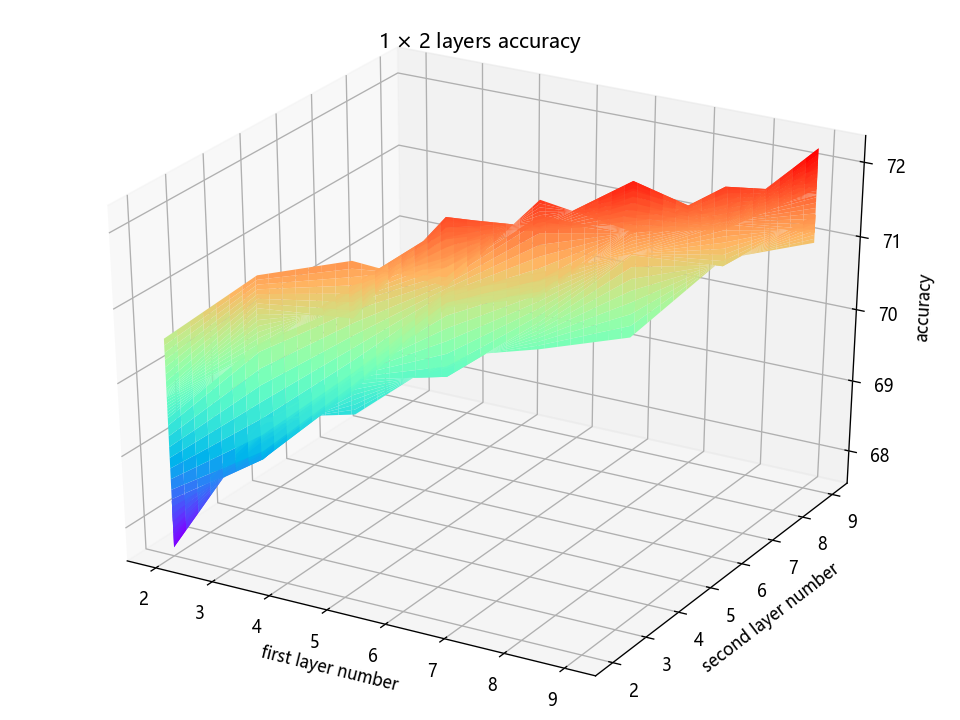
\includegraphics[width=0.5\linewidth, height=0.4\linewidth]{figures/chapter_5/fig_5_16}
		\label{fig_5_6_b}}
	\\
	\subfloat[$H^{(1)} = 2, H^{(2)} = 1$]{
		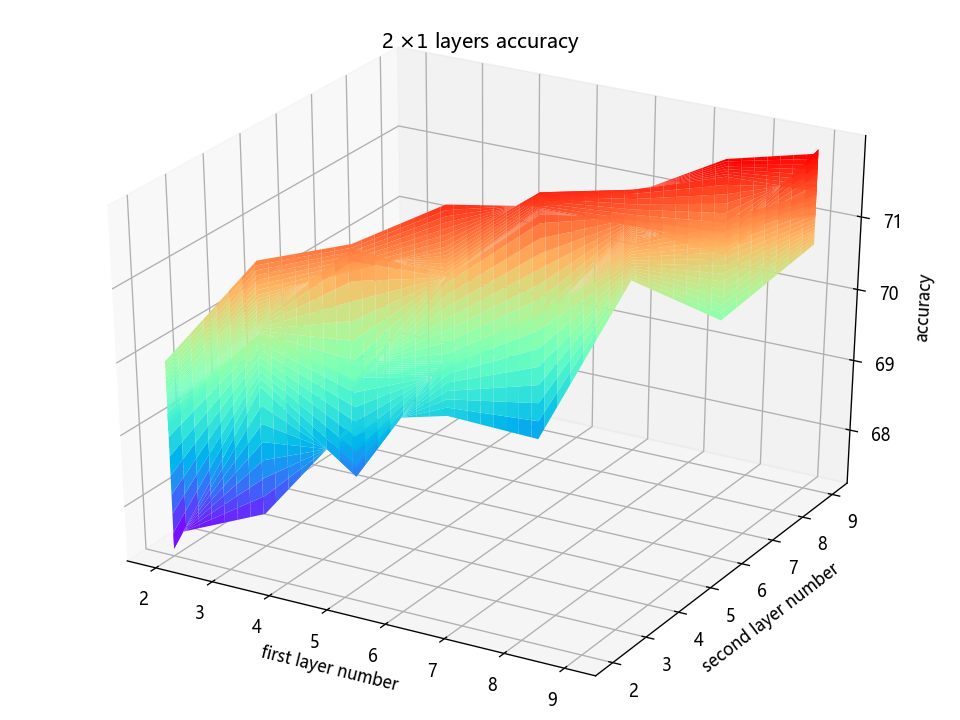
\includegraphics[width=0.5\linewidth, height=0.4\linewidth]{figures/chapter_5/fig_5_17}
		\label{fig_5_6_c}}
	\subfloat[$H^{(1)} = 2, H^{(2} = 2$]{
		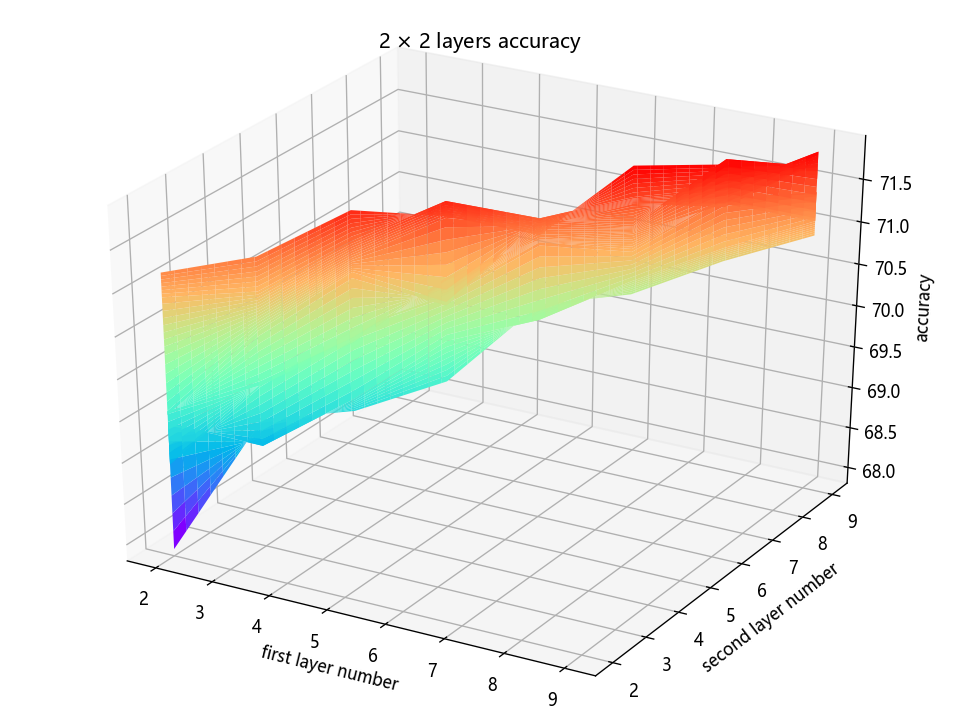
\includegraphics[width=0.5\linewidth, height=0.4\linewidth]{figures/chapter_5/fig_5_18}
		\label{fig_5_6_d}}
	\caption{不同$H^{(1)} \times H^{(2)}$条件下卷积核宽度对分类性能的影响}
	\label{fig_5_6}
\end{figure}

从图\ref{fig_5_6}可以发现一个整体的趋势,即卷积核$W^{(1)}$和$W^{(2)}$小的卷积核性能没有其宽度大的卷积核性能强。
从达到的性能上界而言,图\ref{fig_5_6_b}的最值是超过$72\%$的,高于其他三种情况,
也就是说网络的卷积层高度为$H^{(1)} = 1$,$H^{(2)} = 2$时,模型具有最优分类性能。
这可能是因为随着卷积核的宽度增加,网络变得复杂,模型的容量变大,更能够捕获数据本身所携带的信息,
所以呈现出较宽的卷积核具有较强的分类性能。\par

分类性能在两层高度$H^{(1)}=1$和$H^{(2)}=2$时达到性能上界,
这可能是由于数据本身表示的是信号的$I \times Q$两路的信号,
而 $I$ 路信号与 $Q$ 路信号本身呈希尔伯特变换的关系,
所以,在第一个卷积层利用高度$H^{(1)}=1$的卷积核分别提取每一路的信息,
更符合数据本身逻辑上的关系,因此也更有可能取得好的效果。
\par

从四种情况而言,图\ref{fig_5_6_d}在第二卷积层宽度为$W^{(2)}=3$时分类性能就已经达到一个较高的水平,
相对其他三种情况而言容易更容易达到好的性能;
而图\ref{fig_5_6_a}所示的网络最慢达到一个性能的较高水平。
这可能是由于图\ref{fig_5_6_d}中,卷积核$H^{(1)}=2$和$H^{(2)}=2$,
卷积核宽度大,捕获数据信息能力较强,所以性能较容易在小卷积核时达到较高水平。\par

(2)卷积核宽度对分类准确率影响的二维展示\par 

接下来,通过不同卷积和宽度下的分类准确率的热力图,
来分析卷积核宽度$W^{(1)}$和$W^{(2)}$对分类性能的影响,结果如图\ref{fig_5_7}所示。
\begin{figure}[!h]
	\centering
	\subfloat[$H^{(1)} = 1, H^{(1)} = 1$]{
		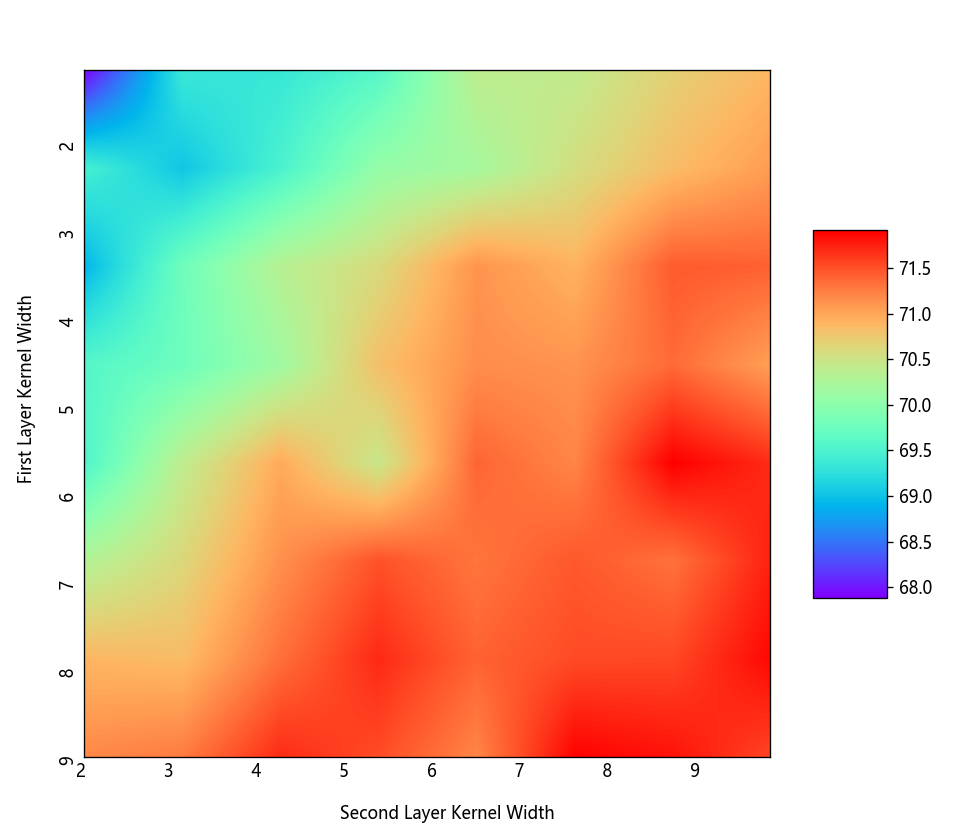
\includegraphics[width=0.5\linewidth, height=0.4\linewidth]{figures/chapter_5/fig_5_23}
		\label{fig_5_7_a}}
	\subfloat[$H^{(1)} = 1, H^{(1)} = 2$]{
		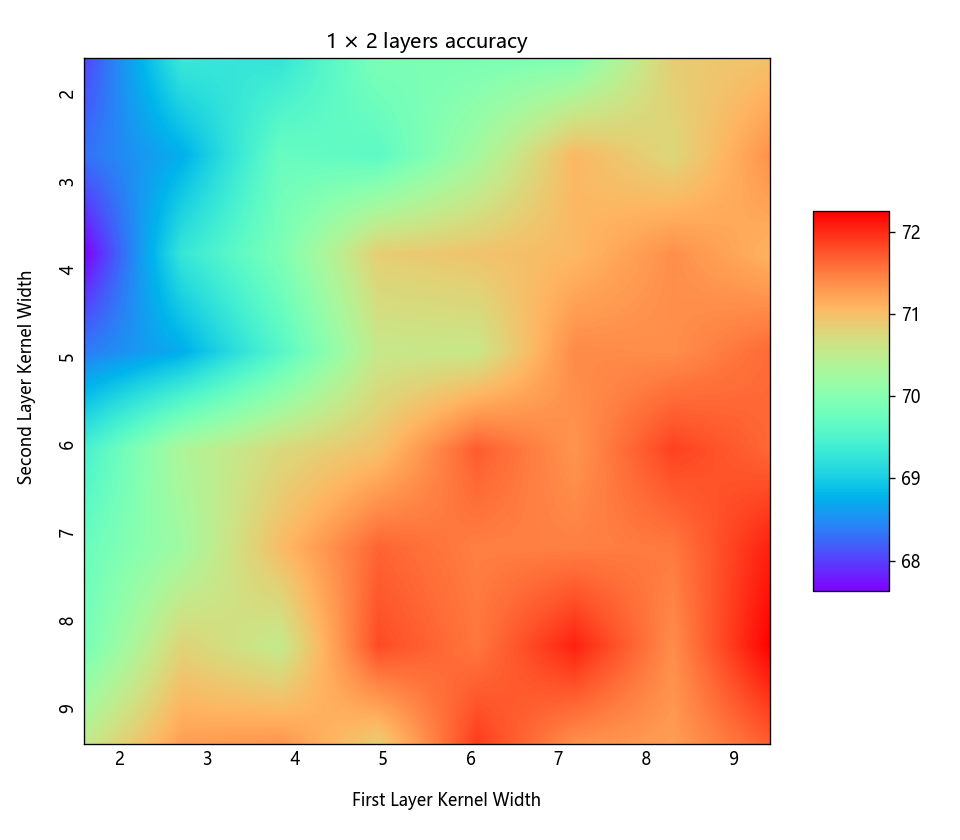
\includegraphics[width=0.5\linewidth, height=0.4\linewidth]{figures/chapter_5/fig_5_24}
		\label{fig_5_7_b}}
	\\
	\subfloat[$H^{(1)} = 2, H^{(1)} = 1$]{
		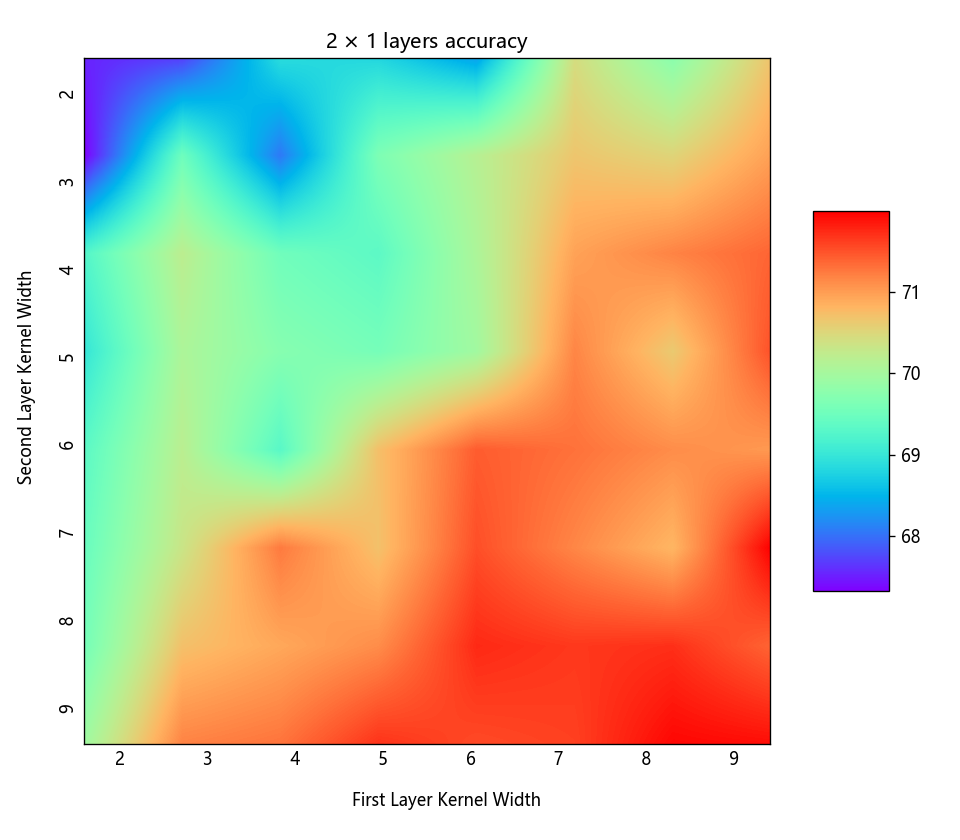
\includegraphics[width=0.5\linewidth, height=0.4\linewidth]{figures/chapter_5/fig_5_25}
		\label{fig_5_7_c}}
	\subfloat[$H^{(1)} = 2, H^{(1)} = 2$]{
		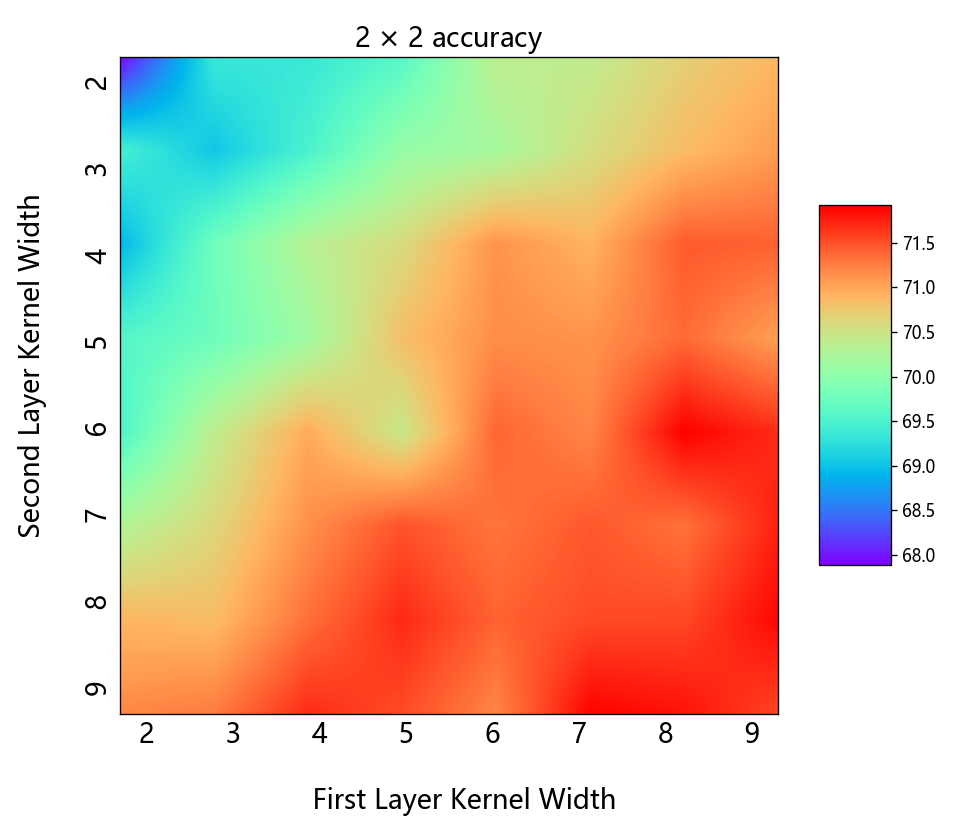
\includegraphics[width=0.5\linewidth, height=0.4\linewidth]{figures/chapter_5/fig_5_26}
		\label{fig_5_7_d}}
	\caption{不同卷积核高度$H^{(1)} \times H^{(2)}$下,卷积核宽度对分类准确率的影响}
	\label{fig_5_7}
\end{figure}

从图\ref{fig_5_7}中可以发现:对卷积核的宽度而言,整体来看较小的卷积核不如较大的卷积核,
但是当卷积的宽度增大到$7$之后,分类性能较为稳定,变化较小。
从图\ref{fig_5_7}中每个子图蓝色的分布而言,可以发现图\ref{fig_5_7_d}占比最小,
即其在卷积核宽度更小时就可以达到较好的性能;
而图\ref{fig_5_7_a}蓝色占比最大,而且颜色较深,所以其只能在卷积核宽度较大时才能达到较好的性能。
这说明卷积核的宽度越大,拟合能力可能越强,获取数据的信息越多。\par

同时,可以看到图\ref{fig_5_7}中各个子图蓝色的分布情况各不相同:
图\ref{fig_5_7_a}和\ref{fig_5_7_d}中蓝色几乎分布在对角线上,
但是图\ref{fig_5_7_a}中$W^{(1)}$的变化对蓝色分布的影响更大一些;
图\ref{fig_5_7_b}中蓝色分布主要沿$W^{(2)}$变化;
图\ref{fig_5_7_c}中蓝色分布主要沿$W^{(1)}$变化。
这说明,如果两个卷积层中卷积核的宽度相同,则改变两个层中卷积核的宽度,
对于分类器的性能影响具有相似性;
但是,可能是因为调制识别的应用场景针对的是$I \times Q$两路信号,当$W^{(1)}=1, W^{(2)}=1$时,
改变$W^{(1)}$对于分类性能影响更大一些。
图\ref{fig_5_7_b}中,由于$W^{(2)}=2$,在卷积核宽度较小时,由于模型处于欠拟合状态,
此时偏差主导了模型的泛化误差,而$W^{(2)}$的增加对于网络容量提升更快,
因此,改变$W^{(2)}$会取得更好的性能提升。图\ref{fig_5_7_c}的现象,可能也是这种原因。\par
%\section{常见的网络架构}
%LeNet主要是用于识别10个手写数字的,但其具有较简单的网络底层结构,对于复杂数据识别效果较差。
%自2012年ImageNet竞赛之后,深度学习在之后大放异彩,表\ref{sec:table_5_1}是近几年主流的深度框架(AlexNet、VGG、GoogLeNet、ResNet)的比较。\par
%\begin{table}[H]\label{sec:table_5_1}
%	\centering
%	\caption{ ILSVRC历年Top-5错误率}
%	\begin{tabular}{ccccc}
%		\toprule
%		模型 & AlexNet & VGG & GoogLeNet & ResNet\\
%		\midrule
%		发布时间 &	2012 & 2014 & 2014 & 2015\\
%		\midrule
%		层数 & 8 & 19 & 22 & 152\\
%		\midrule
%		Top-5错误率 & 16.4\% & 7.3\% & 6.7\% & 3.57\%\\
%		\bottomrule 
%	\end{tabular}
%\end{table}
%AlexNet相比传统的CNN的改进主要在数据增强、dropout、池化、ReLU函数等,相较于我们提出的CNN基础框架没有本质上的区别。
%而VGG主要的改进是网络深度的改进,对我们的调制数据而言,网络深度的增加并不能带来模型性能的提升。
%因此,本文中我们对其影响并不作研究,而是主要对几个主流框架GoogLeNet、ResNet、CLDNN的底层结构进行改动适应调制信号的维度,
%并降低网络深度,观察不同的底层网络结构对调制识别的影响。
%
%\subsection{InceptionNet}
%GoogLeNet相较于CNN主要的创新在于提出了Inception结构,这是一种底层的网络结构,其类似于卷积核一样,是一种网络组成的单元。
%它可以提高网络深度和宽度,并能够将不同规模的特性推广到一般管理复杂性。
%Inception一直在不断发展,目前已经发展到$v4$版本,对于我们的调制识别应用场景,
%经过修改后基本的网络结构如图\ref{fig_5_4}所示:\par
%\begin{figure}[!h]
%	\centering
%	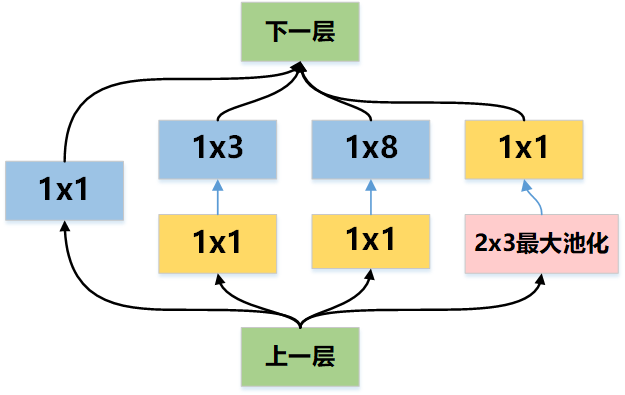
\includegraphics[scale=0.8]{figures/chapter_5/fig_5_27}
%	\caption{InceptionModel}\label{fig_5_27}
%\end{figure}
%每个Inception模块(如图\ref{fig_5_4}所示)包含四条并行路径,输出是四个并行输出的串联,
%用了Inception结构之后整个网络结构的宽度和深度都可扩大。
%第一条路径是一组对选定信息转发的$1\times1$卷积核,它只是简单地向前传递信息而不进行变换,
%可以使选择性信息高速前向传播。
%第二和第三条通道首先是$1\times1$卷积,接着是一组$1\times3$和$1\times8$卷积以提供多个宽度的特征检测。
%最后一条并行通道,首先是一个3x3池化层,接着是1x1卷积。\par
%我们在特征提取层中使用了两层适应性重构后的Inception网络,其中第一层包含32个Inception结构,第二层包含16个Inception结构。
%这样,我们可以保证在尽量不提高网络深度和宽度的情况下,学习数据的不同维度特征。\par
%
%\subsection{残差网络}
%残差网络(ResNet)的提出本质上是要解决层次比较深的时候无法训练的问题。
%使用跨层转发信息的体系结构是一种增加网络深度的有效方法,
%微软凭借ResNet的网络结构增加网络层深度至152层并赢得ImageNet 2015的冠军[4]。
%这种借鉴了Highway Network思想的网络相当于在主干网络之外开通一个特殊通道使得输入可以直达输出。
%图\ref{fig_5_5}展示了ResNet的基本结构:\par
%\begin{figure}[!h]
%	\centering
%	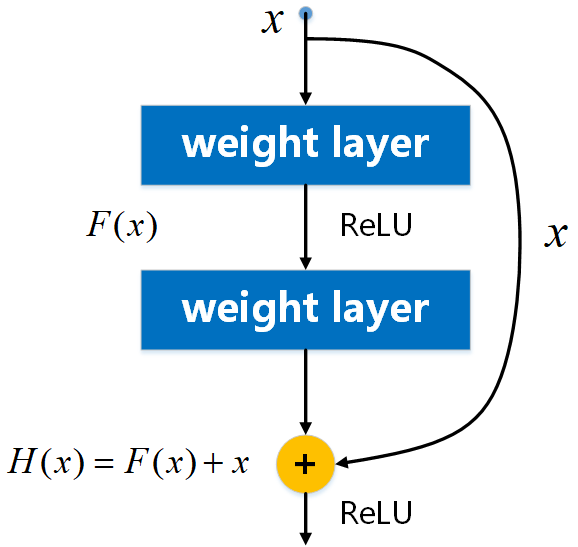
\includegraphics[scale=0.6]{figures/chapter_5/fig_5_28}
%	\caption{残差网络结构}\label{fig_5_28}
%\end{figure}
%如图\ref{fig_5_5}所示,,$x$是网络的输入,主干网络为输入信号$x$经过不同的网络层后向传播;
%同时,ResNet也会将一层的输出添加到更深层的两层输出中。
%其中$H(X)$是某一层原始的的期望映射输出,而优化的目标由原来的拟合输出$H(x)$变成输出和输入的差$H(x)-x$,
%由于ResNet的信息转发迫使网络学习残差函数进而学习数据的特征,因此这样的网络结构被称之为残差网络。\par
%ResNet的作者认为消失梯度可以通过广泛采用的归一化技术来解决,而深度网络的深度则受限于深度网络的训练复杂度,
%而残差网络正可以通过额外的信息转发通道,弱化网络深度对训练复杂度的影响。\par66
%
%由本章第二小节得到的结论,网络的深度并不是我们调制性能限制的主要因素。
%因此,我们在ResNet调制识别网络的设计时,仅仅考虑到使用五个层的简单网络,每隔两层进行信息转发,
%来探索ResNet的网络结构是否能提高调制识别的准确率。
%
%
%\subsection{卷积长短期深度神经网络}
%CNN可以减小频率的偏移变化,LSTM则很适合对时序语音进行建模,DNN就可以对特征进行非线性映射到一个抽象空间进行有效分离。
%卷积长短期深度神经网络(Convolutional Long short-term Deep Neural Networks,CLDNN)正是一种将CNN、LSTM和DNN结合的用于语音处理的算法。它在CNN上加入了对输入特征的时域卷积,同时实现了时域和频域卷积,并将时频域上的特征进行关联。\par
%
%受通信领域专业知识引导和CLDNN等网络体系结构的启发,我们最朴素的想法是采用典型通信接收器的通用结构,
%并构建具有类似结构的神经网络。
%通信接收机有一个卷积核(通常与传输的脉冲或波形匹配),同步器和采样器。
%通常,前置卷积核抽取每个符号的少量采样,用于执行相移以找到最佳采样点的同步器。
%与此类似的神经网络体系结构是卷积层,因此我们首先引入卷积层。
%LSTM广泛用于时间序列应用,由于我们是对时间序列信号进行分析获取调制方式,
%需要对时间特征进行建模,因此我们引入了LSTM单元组成的层。
% \par
%本论文中使用的CLDNN结构如图\ref{fig_5_29}所示:\par
%\begin{figure}[!h]
%	\centering
%	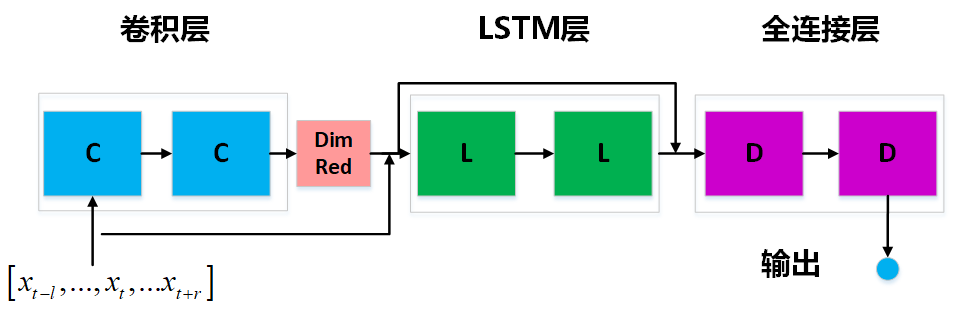
\includegraphics[scale=0.6]{figures/chapter_5/fig_5_29}
%	\caption{CLDNN结构}\label{fig_5_29}
%\end{figure}
%我们测试了两层和三层卷积的CLDNN型结构,其功能类似于卷积匹配卷积核。
%而在,由于数据本身不具备较高的复杂度,我们采用了两层的版本,实际证明两个卷积层的网络性能相对更优。
%随后是两个由长期短期记忆(LSTM)单元组成的循环层,其主要用于建模数据的时间特征。
%由于调制基带数据是时间序列,因此我们认为这对于整体的网络来说可能是一个较优的改进。
%CLDNN也可以具有绕过层的连接,旨在为数据提供更长的时间上下文信息。
%例如,原始CLDNN在LSTM层之前转发卷积层输出的原始样本到DNN层,此连接是原始波形和卷积输出的连接。
%我们尝试过有和没有前向连接,发现加入连接之后,网络的分类精度更高,梯度下降更稳定。\par
%
%\section{结果及分析}
%
%本节中,我们继续使用第三章中的数据集作为评估调制识别性能的基础。
%我们使用所有信噪比条件下的$top-1$分类精率作为单个数字基准,并且比较信噪比在0dB时的分类精度。
%所有模型的训练都基于Tensorflow深度学习库,平台系统配置如表\ref{sec:table_3_1}所示。\par

%
%\subsection{GoogLeNet分类混淆矩阵}
%
%\subsection{ResNet分类混淆矩阵}
%
%\subsection{CLDNN分类混淆矩阵}
%
%为了进一步理解什么限制了分类的准确性,我们看一下图1所示的CLDNN的混淆矩阵。 8.有两个主要的混淆领域。一个在模拟调制之间,另一个在高阶QAM之间。模拟调制将很难解决,但是QAM可以通过更好的同步和减少信道损伤来改善。
%对CLDNN在每一层学习的内容有直觉,对指导未来的工作很重要。为此,我们绘制了一些卷积核抽头的时间和频率表示。对于频率响应,卷积核抽头用零填充100个零点以获得128点FFT。图图9a和图10a示出了来自第一层的两个选择卷积核。专家的眼睛看起来并不特别熟悉时域表示;然而频率响应确实显示了整形的低通卷积核。未示出的其他卷积核具有频率选择性组件,DC阻断器和类似sinc的频谱形状。
%
%为了进一步理解什么限制了分类精度,我们查看了图10中所示的CLDNN的混淆矩阵。有两个主要混淆领域。 一个在模拟调制之间,另一个在高阶QAM之间。 模拟调制将很难解决,但是QAM可以通过更好的同步和减少信道损伤来改善。\par
%
%为了进一步理解什么限制了分类的准确性,我们看一下图8所示的CLDNN的混淆矩阵。有两个主要的混淆领域。一个在模拟调制之间,另一个在高阶QAM之间。模拟调制将很难解决,但是QAM可以在更好的同步和减少信道损伤的情况下得到改善。\par
%
%
%我们的超参数优化CNN和9层残留网络达到了相似的损失,验证损失和准确性,但未显示;然而,剩余网络在更少的时期学习。我们还试验了5-9层的残留网络,它们都具有相似的性能和训练时间。这与我们对普通CNN深度的超参数搜索相结合,表明我们不受无线电学习任务网络深度的限制,尽管我们受到纯粹CNN架构可以学习的功能的限制。\par

\section{本章小结}

本章从网络底层研究网络超参数对调制识别性能的影响,
并从欠拟合与过拟合以及偏差与方差的角度来理解出现这些现象的原因。
CNN在调制识别时的性能似乎不受网络深度的限制,在卷积层数目为$3$时即可达到性能的最值,
此时再增大卷积层的深度,系统性能可能会发生下降。
第一层卷积核数目较小时,
网络的性能几乎随着第二层卷积核数目的增大而减小。
而随着第一层卷积核增大,改变第二层卷积核数目,系统分类准确率变化很小,只有轻微的波动;
卷积核数目$N_{kernel}^{(1)} =64, N_{kernel}^{(2)} =48$时,系统取得所能观察到的最好性能;
当$N_{kernel}^{(1)}$较小时,增大$N_{kernel}^{(2)}$到超过第一个卷积层的核数目时,模型的性能会下降。
整体而言,卷积核宽度$W^{(1)}$和$W^{(2)}$小的卷积核性能没有宽度大的卷积核性能强,
但是当卷积的宽度增大到$7$之后,分类性能较为稳定,变化较小;
卷积核的高度$H^{(1)}$和$H^{(2)}$不同时,改变每一层的卷积宽度对系统造成的影响不同,
相对而言,改变高度$H$大的卷积核对系统的性能影响较大。\par
